%================================================================================================% 
% thesis.tex                                                                                     %
% This is the main file, which calls up preamble.tex, front-matter.tex, and thesis.bib as needed. %
%================================================================================================%

% Front-matter shortcuts; note the extra space at the end, which is unfortunately necessary:      
\newcommand\myname{John P Gallagher }
\newcommand\mytitle{AN ERDOS SIMILARITY PROBLEM IN A TOPOLOGICAL SETTING } % The graduate division requires this to be in caps.
\newcommand\mydegree{Master of Arts } % change to  Master of Science if applicable
\newcommand\myfield{Mathematics } % e.g., Mathematics
\newcommand\thismonth{May } % graduation month: May / August / December
\newcommand\thisyear{2022 } % e.g., 2014

\newcommand\myadviser{Dr. Chun-Kit Lai} % Adviser
\newcommand\myadviserstitle{Associate Professor}
\newcommand\committeememberone{Dr. Emily Clader} % Committee member 1
\newcommand\committeememberonetitle{Assistant Professor} 
\newcommand\committeemembertwo{Dr. Arek Goetz} % Committee member 2
\newcommand\committeemembertwotitle{Professor}

\documentclass[12pt,oneside]{sfsuthesis}  
%WHEN THESIS IS COMPLETED, CHANGE THE NEXT LINE FROM draft TO final, then the paper will be formatted according to the Graduate Division's guidelines
\usepackage[final]{MAThesisOutputFormat}
\RequirePackage{standalone}

%==========%
% biblatex %
%==========%

\usepackage[backend=biber,style=numeric]{biblatex}
\addbibresource{thesis.bib}

%=========================%
% CUSTOM PACKAGES GO HERE %
%=========================%

%\usepackage{TCbasic}

\begin{document}
\thesistitle
% Main body of work:
\chapter{Introduction}

From the perspective of applied math, empirical results are almost always discrete observations yet the relationships that are observed are not necessarily quantized.  This means that as we infer mathematical relationships from discrete sets, there can often be a mismatch between our theoretical model, and the true relationships.  This notion of embedded relationships is also a core area of study within pure mathematics.  Whether observing a pattern and trying to generalize the relationship to a broader context, or deducing a relationship from a different set of assumptions, discrete patters are intrinsically embedded in our universe.  Indeed as we examine our world we often notice similarities we want to measure.  Using that same measure we want to look for consistency, and should we see something similar to our original observation we would expect a similar measure.  

However in mathematics (and life), the rules we construct often lack the subtly to account for nuances. Let us na\"{i}vely consider measurement.  Suppose we have a string and want to find out its length.  After pulling the string taught along a ruler, we might see it is a few centimeters long.  Then from this collection of tools we might say that we only need two points and a ruler to be able to describe length.  In reality we have only learned of distance.  

From that same construction though, we could just as well say, 2 points have no length at all because there is nothing between them.  In a sense, both are simultaneously true, because our definition does not address these nuances.  This motivates a few new questions: How many points do you need to add in, before we can have a length of string?  Can we use this string to measure other things?  Can we use collections of points to measure other things?  And maybe strangest of all, can collections of points have the same length as a piece of string?

We can now go back to our notion of the universe and ask ourselves these questions again.  Suppose we change universes, does our notion of length still exist? In a different universe can we find similar copies of these collections of points? 

Key words:\begin{itemize}
    \item Dynamical Systems
    \item Density and Measure are not clearly linked
    \item Geometry
    \item Fractals poorly defined
    \item Self Similarity is more well defined
    \item Cantor Set
    \item $\R^n$ Fractals
    \item Erd\"{o}s Proposed Conjecture with Measure Space assumptions
    \item Theorem with Topological Assumptions.
    \item Open questions
\end{itemize}

%\section{Introduction to the Introduction}



%\subsection{Introduction to the Introduction to the Introduction}



% main.tex, to be used with thesis.tex
% This contains the main work of your thesis.
\chapter{Introduction}

Here's where you text starts. You might (but don't have to) have sections like\dots

\section{Introduction to the Introduction}

\dots or subsections\dots

\subsection{Introduction to the Introduction to the Introduction}

To include text in your document, you just type. You don't have to worry about spacing between sentences; \LaTeX \ does that automatically. 
To start a new paragraph, just insert an empty line.

Here comes the new paragraph. You can include tables, such as Table \ref{tablename}, which can also be turned if necessary, as seen, e.g. in Table~\ref{tablenameturned}. (I
think the latter is automatically on its own page; the former will just be put where \LaTeX \ thinks it fits best.)

\begin{table}[htb]
\begin{center}
\begin{tabular}{c||r|r|r|r|r|r|r|r}
$d$ & 2 & 3 & 4 & 5 & 6 & 7 & 8 & 9 \\ 
\hline
\text{bound} & 3.6 & 8.5 & 15.8 & 25.7 & 38.3 & 53.5 & 71.4 & 92.0
\end{tabular}
\end{center}
\caption{Bounds in various dimensions $d$.}
\label{tablename}
\end{table}

\begin{sidewaystable}
\begin{center}
\begin{tabular}{c||r|r|r|r|r|r|r|r}
$d$ & 2 & 3 & 4 & 5 & 6 & 7 & 8 & 9 \\ 
\hline
\text{bound} & 3.6 & 8.5 & 15.8 & 25.7 & 38.3 & 53.5 & 71.4 & 92.0
\end{tabular}
\end{center}
\caption{More bounds in various dimensions $d$.}
\label{tablenameturned}
\end{sidewaystable}

To start a new chapter, you don't need to add a page break\dots

\chapter{The Real Stuff}

\dots \LaTeX \ does that automatically.

\section{Various Tricks}

Here are a few tidbits that came to my mind, in no particular order\dots

I'm sure most people know about {\tt $\backslash$label} and {\tt $\backslash$ref}; this feature is enough reason for me to use \LaTeX. 
For example, you might have something like\dots

\begin{theorem}[Euler]\label{eulerthm}
Leonhard says $e^{ 2 \pi i } = 1$.
\end{theorem}

\dots which you can then later (or earlier) reference as Theorem \ref{eulerthm} and you can point to page \pageref{eulerthm} on which it appears.
If you label equations like
\begin{equation}\label{eulereq}
  e^{ 2 \pi i } = 1 \, ,
\end{equation}
you can reference them most lazily using \eqref{eulereq}.

\def\v{{\mathbf v}}
\def\P{{\mathcal P}}
\def\Z{\mathbb{Z}}
\newcommand\floor[1]{\left\lfloor {#1} \right\rfloor} 

There are two ways to define internal macros: {\tt $\backslash$def} and {\tt $\backslash$newcommand}. The difference is that the former overwrites any possibly existing command,
where as the latter induces a \LaTeX \ complaint if you're redefining an existing command (in which case you should use {\tt $\backslash$renewcommand} instead). Since I'm lazy,
I tend to use {\tt $\backslash$def}, with one important exception: {\tt $\backslash$newcommand} allows you to use arguments. For example, the definition
\begin{verbatim}
\newcommand\floor[1]{\left\lfloor {#1} \right\rfloor} 
\end{verbatim}
produces a flexible floor function $\floor{\frac{ 3\pi }{ 2 }}$. And yes, the {\tt [1]} can be replaced by {\tt [n]} if you have use for {\tt n} arguments (which get the
placeholders {\tt \#1}, {\tt \#2}, \dots, {\tt \#n}).

The previous example reminds me to strongly recommend the use of {\tt $\backslash$left} and {\tt $\backslash$right} whenever you use parentheses:
\[
  ( \frac a b - 2 ) \ \text{ just doesn't look good compared with } \ \left( \frac a b - 2 \right) .
\]

There are three dashes in \LaTeX---one like the one you just saw, one that's used in ``Berndt--Zaharescu's Theorem" or ``Chapter 7--9," and one that's used in ``well-known
identity."

\newcommand{\todo}[1]{\par \noindent
  \framebox{\begin{minipage}[c]{0.95 \textwidth} TO DO:
      #1 \end{minipage}}\par}

One of my favorite packages is {\tt enumerate}:
\begin{enumerate}[{\bf i)}]
  \item first item
  \item second item
  \item third item
  \item \dots
\end{enumerate}

\todo{I stole the idea of a to-do box from a friend. This is useful when editing a paper and you want to remind your co-author or yourself about something\dots}

%%%%%%%%%%%%%%%%%%%%%%%%%%%%%%%%%%%%%%%%%%%%%%%%%%%%%%%%%%%%%%%%%%%%%%%%%%%

\section{Math}

You can put a $\Box$ at the end of a math line if a proof happens to end with a math line. The version\dots

\begin{proof}
This follows from
\[
  e^{ 2 \pi i } = 1 \, .
\]
\end{proof}

\noindent
\dots wastes space and doesn't look nearly as cool as\dots

\begin{proof}
This follows from
\[
  e^{ 2 \pi i } = 1 \, . \qedhere
\]
\end{proof}

Speaking about proofs, sometimes you need a paragraph or two between a theorem and its proof, in which case you can use\dots

\begin{proof}[Proof of Theorem \ref{eulerthm}]
This follows from
\[
  e^{ 2 \pi i } = 1 \, . \qedhere
\]
\end{proof}

\def\lcm{\operatorname{lcm}}

You can (and should) define your own math operators with {\tt $\backslash$operatorname}. For example,
\[
  \lcm (2, 3) = 6 \ \text{ looks better than } \ lcm (2, 3) = 6 \, .
\]
Speaking about lcm's, I find it amusing that {\tt $\backslash$gcd} is a pre-defined operator, whereas {\tt $\backslash$lcm} is not. 

The {\tt $\backslash$dots} command is relatively smart in \LaTeX; e.g., it knows automatically where to put the dots in $\left\{ 1, 2, \dots, n \right\}$ as compared to $1 + 2 +
\dots + n$.
If you ever need to force a certain alignment of the dots, use $\ldots$, $\cdots$, $\vdots$, or $\ddots$.

For math stuff that takes several lines I prefer the environment {\tt align} over {\tt eqnarray}. The difference is minor but I still prefer
\begin{align*}
  \sum_{ j=1 }^{ k-1 } \chi(j) \sin^2 \left( \frac{ \pi j }{ k } \right) \tan \left( \frac{ 2 \pi j }{ k } \right)
  &= \sqrt k \left( - \frac 1 2 + \left( \chi(2) - 2 \right) h(-k) \right) \\
  &= \begin{cases}
      \sqrt k \left( - \frac 1 2 - 3 \, h(-k) \right) & \text{ if } k \equiv 3 \bmod 8 , \\
      \sqrt k \left( - \frac 1 2 - h(-k) \right) & \text{ if } k \equiv 7 \bmod 8
    \end{cases}
\end{align*}
over
\begin{eqnarray*}
  \sum_{ j=1 }^{ k-1 } \chi(j) \sin^2 \left( \frac{ \pi j }{ k } \right) \tan \left( \frac{ 2 \pi j }{ k } \right)
  &=& \sqrt k \left( - \frac 1 2 + \left( \chi(2) - 2 \right) h(-k) \right) \\
  &=& \begin{cases}
      \sqrt k \left( - \frac 1 2 - 3 \, h(-k) \right) & \text{ if } k \equiv 3 \bmod 8 , \\
      \sqrt k \left( - \frac 1 2 - h(-k) \right) & \text{ if } k \equiv 7 \bmod 8 .
    \end{cases}
\end{eqnarray*}

%%%%%%%%%%%%%%%%%%%%%%%%%%%%%%%%%%%%%%%%%%%%%%%%%%%%%%%%%%%%%%%%%%%%%%%%%%%

\section{Graphics}

My favorite way to produce graphics is through a (public-domain) program called {\tt jPicEdt}; it produces \LaTeX\
code that can be read right into the file (using the {\tt $\backslash$input} command).
My second favorite way to go about graphics is through the package {\tt graphicx}. I produce my graphics with a separate program, export them into pdf, and then overlay them
with \TeX\ symbols if needed; see Figure \ref{intrographfig} for an example.

\begin{figure}[htb]
\begin{center}
\begin{picture}(60,60)
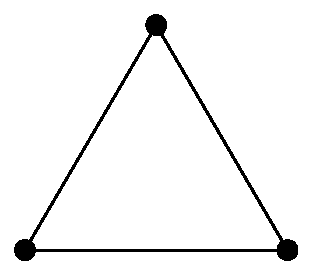
\includegraphics[totalheight=.8in]{intrograph}
\end{picture}
\begin{picture}(0,0)
  \put(-157,0){$t-1$ color choices}
  \put(-22,50){$t$ color choices}
  \put(5,0){$t-2$ color choices}
\end{picture}
\end{center}
\caption{Proper $t$-colorings of $K_3$.}\label{intrographfig}
\end{figure}

The overlaying of figures reminds me of two of my other favorite \LaTeX \ commands: {\tt $\backslash$vspace} and {\tt $\backslash$hspace}. For example, they allow you to place
just about

\vspace{.5in}
\hspace{2in}
anything

\vspace{-.5in}
\hspace{5in}
anywhere.

\vspace{.5in}
\noindent
This can be very useful, e.g., for presentations in which you might move pictures around.

%%%%%%%%%%%%%%%%%%%%%%%%%%%%%%%%%%%%%%%%%%%%%%%%%%%%%%%%%%%%%%%%%%%%%%%%%%%

\section{Bibliographic Stuff}

For references like \cite[Section 2]{athanasiadismagic} I recommend using {\tt bibtex}; it means that you have to do only minimal work, especially when you get the entries
from \emph{MathSciNet}. I keep all the references I've ever used in the same file and use this in all my documents\dots

If you could use an index at the end of your document, use {\tt makeindex}---one of best reasons to use \LaTeX \ if you're writing a book.




\section{A Cantor set with positive Newhouse Thickness is not universal}
We  say that a set $E$ is  {\it universal} in the collection of dense $G_{\delta}$ sets if for all $G_{\delta}$ set,  we can  always find some affine copies of $E$ inside the set. By an affine copy, we  mean sets of  the form $t+\lambda E$ for some $t\in{\mathbb R}$ and $\lambda\ne 0$. A natural question we have is that  is there a nowhere dense Cantor Set that is universal in the collection of dense $G_\delta$ sets? This is an exploration of an Erd\"{o}s conjecture in a topological setting. 

\begin{theorem}\label{theorem_positive_NW}
Let $J$ be a cantor set with positive Newhouse thickness.  Then $J$ is not universal.
\end{theorem}

\begin{proof} Suppose we have some Cantor set $J$ with Newhouse thickness $\tau(J) >0$. Without loss of generality, we  can assume  the convex hull of $J$ $[0,1]$.   Consider Cantor sets $K$ defined by contraction ratio $1/N$ and digits $\{0,1,...,N-1\}\setminus\{(N-1)/2\}$ and $N$ is odd. By a simple calculation,  $\tau (K) = \frac{N-1}{2}$. Therefore,  we can find a  sufficiently large $N$ so that $\tau(J)\tau(K)>1$. 

\medskip

Using the Cantor set $K$ Define $X$ such that $$
X = \bigcup_{n \in \Z} \bigcup_{\ell \in \Z} N^n(K+\ell),
$$creating a dense $F_\sigma$ set. Now consider $X^c$.  Because $K^c$ is open and dense and so is its translated and dilated copies, by the Baire Category Theorem, $X^c$ is a dense $G_{\delta}$.  We now show that $X^c$ contains no affine copy of $J$. 

\medskip

Suppose we have some affine copy, $t+ \lambda J$ where $t\in\R$ and $\lambda\ne 0$. There exists a unique $n$ such that 
\begin{equation}
    |\lambda| \in (N^{n-1}, N^n].
\end{equation}
Similarly there exists a unique $\ell$ such that 
\begin{equation}
t \in (\ell  N^n, (\ell+1)N^n].    
\end{equation}
We claim that this affine copy of $J$ has a non-empty intersection with $N^n(K+\ell)$.  This is equivalent to  showing that 
$$t \in N^n(K+\ell)-\lambda J.$$
For consistent notation with a referenced theorem, let 
$$C_1 = N^n(K+\ell) \text{ and } C_2 = - \lambda J.$$
First we check the construction of our Cantor sets. For $C_1$ its largest corresponding open gap interval is $|O_1| = N^{n-1}$ and its largest corresponding closed interval is $|I_1| = N^n$. For $C_2$ and is corresponding intervals, we find that $|O_2| =|\lambda|\cdot |O_J| \le |\lambda|$ and $|I_2| = |\lambda|$ where $O_J$ is the largest  open gap interval in $J$.  Therefore by our construction in (1) the following two inequalities hold: $$|O_1|\leq |I_2| \text { and } |O_2| \leq |I_1|$$ as in the condition of Theorem 2.2.1 in \cite{Astels}.  By \cite [Theorem 2.2.1]{Astels}\footnote{This might misattribute the theorem.  I think Astels '99 Theorem 2.2.1 is  actually is quoting Newhouse directly.  In particular I think it refers to Newhouse 1979 \cite{PMIHES_1979__50__101_0} \textit{The Abundance of Wild Hyperbolic Sets, and Non-smooth Stable Sets for Diffeomorphisms}. }, given that the Newhouse thickness of our sets, $\tau(K)\tau(J) \geq 1$ then $C_1 + C_2 = I_1 + I_2$. Note that   $I_1 = [\ell N^n, (\ell+1)N^n]$,  $I_2=[-\lambda, 0]$ if $\lambda>0$  and $I_2=[0,-\lambda]$ if $\lambda<0$.  we find that 
$$
I_1+ I_2 = [N^n\ell - \lambda, N^n(\ell+1)] \  (\lambda>0) \ \mbox{and} \ I_1+I_2 = [N^n\ell, N^n(\ell+1)-\lambda] (\lambda<0).
$$
Then from (2)
$$t \in I_1+I_2.$$
Therefore the affine copy of the cantor set $t + \lambda J$ has a non-empty intersection with $X$ and $J$ cannot be universal.

\end{proof}

It would be interesting to study those Cantor sets with Newhouse thickness zero. We do not  know what would happen. However, it seems like if we assume a weaker condition on $J$. 

\medskip

\noindent $(\ast):$ There exists $K$ such that $J+K = I_J+I_K$, where $I_J,I_K$ are the  smallest closed interval containing $J$ and $K$. 

\medskip

we  may be able to show that  $J$  cannot be  universal for dense $G_{\delta}$ sets. 

\section{Current Research Questions: Zero Newhouse Thickness} 
%Here are a few notes from today's meeting.  In particular we are now exploring adjacent problems, and trying to understand more properties of our construction, and which portions of our theorem are sufficient, necessary, and unnecessary.  
This section is devoted to study  if Cantor sets with zero Newhouse thickness can be universal. We first  provide an example for  which two Cantor sets with zero Newhouse thickness can still have arithmetic sum equal  to an interval,  showing that the converse of theNewhouse thickness theorem us  not true.   %is one example where we construct two appropriate cantor set with zero Newhouse thickness that combine to create an interval. 
%One question we have about Newhouse Thickness: Can we repeat the same process as above but with Newhouse Thickness $0$?  That is to say, positive Newhouse thickness is sufficient condition for our theorem.  As a refinement, what are the necessary conditions for a Cantor set to not be universal? 
\begin{example}
{\rm Let $N_1, N_2, \dots \in \N_{\geq 2}$. Consider the following construction of a Cantor set using a decomposition of the unit intervals. }
$$\begin{aligned}
[0,1] = &\frac{1}{N_1}\{0,1, \dots, N_1-1\} + \left[0,\frac{1}{N_1}\right]\\
 = & \frac{1}{N_1}\{0,1, \dots, N_1-1\} + \frac{1}{N_1 N_2}\{0,1, \dots, N_2-1\} + \left[0,\frac{1}{N_1 N_2}\right]\\
 =&...\\
 =&\frac{1}{N_1}\{0,1, \dots, N_1-1\} +  \frac{1}{N_1 N_2}\{0,1, \dots, N_2-1\} + \dots + \frac{1}{N_1 \cdots N_n} \{0,\dots, N_n \}+ \dots
\end{aligned}$$
{\rm From here we can define the two cantor sets $K_1, K_2$ where $K_1$ constitutes the odd indices sets in the above summands and $K_2$ has the even one.   This gives the following constructions for the two Cantor sets: }
$$K_1 = \frac{1}{N_1}\{0,1, \dots, N_1-1\}  + \dots + \frac{1}{N_1 \cdots N_{2n+1}} \{0,\dots, N_{2n+1}-1 \}+ \dots$$
$$K_2 = \frac{1}{N_1N_2}\{0,1, \dots, N_2-1\}  + \dots +\frac{1}{N_1 \cdots N_{2n}} \{0,\dots, N_{2n}-1 \}+ \dots$$
{\rm From this construction we see that $K_1 + K_2 = [0,1]$ is the interval but from the definition of Newhouse thickness, }
$$\tau(K_1) = \inf \left\{\frac{1}{N_1-1}, \frac{1}{N_3-1},\dots\right\} = 0 $$
$$\tau(K_2) = \inf \left\{\frac{1}{N_2-1}, \frac{1}{N_4-1},\dots\right\} = 0.$$
{\rm Therefore we have created an interval from two sets with Newhouse thickness $0$ if we have $\lim_{n\to\infty} N_n = \infty$. }
\end{example}
\vspace{0.5cm}  

%The next steps are explorations on which conditions are sufficient, and which conditions are necessary.  

We ask the following questions. Recall $I_J$ denotes the smallest closed interval containing the Cantor set $J$ and $O_J$ denotes  the largest open interval in $I_J\setminus J$. 


\begin{enumerate}
    \item Given a Cantor set $J$, does there exist some $K$ such that $J+K = I_J + I_K$?
    \item If we assume that there exists $K$ such that  $J +K = I_j + I_K$, can we prove that $J$ is not universal?
    \item (rescaling condition) If we assume that $|\lambda_1 I_J| \geq |\lambda_2 O_K|, |\lambda_2 I_K| \geq |\lambda_1 O_J|$ and  $J +K = I_J + I_K $, then $ \lambda_1 J + \lambda_2 K = \lambda_1 I_J + \lambda_2 I_k$.
\end{enumerate}

We also notice that to solve the second question, we notice that $J+K = I_J+I_K$ implies that 
$$
(J+a)+(K+b) = (I_J+a)+(I_K+b) \ \mbox{and} \  bJ+bK = bI_J+bI_K.
$$
We can always translate and rescale $J,K$ so that $I_J = [0,a]$ and $I_K = [0,1]$. Moreover, the following lemma is important. 

\begin{lemma}\label{lemma_gap}
Suppose that the Cantor sets $J$ and $K$ satisfies $J +K = I_j + I_K$. Then $|I_J| \ge |O_K|$ and $|I_K|\ge |O_J|$.
\end{lemma}

\medskip

The lemma also said that  the condition $|\lambda_1 I_J| \geq |\lambda_2O_k|, |\lambda_2 I_k| \geq |\lambda_1 O_J|$ is necessary in the rescaling  condition. 

\medskip

\begin{proposition}
Let $J$ be a Cantor set such that $J+K = I_J+I_K$ where $I_J = [0,a]$ and $I_K = [0,1]$. Suppose that the rescaling condition (3) holds. Then $J$ is not universal in the collection of dense $G_{\delta}$. 
\end{proposition}

\begin{proof}
The proof is similar to the proof in Theorem  \ref{theorem_positive_NW}. With $K$ given in the assumption. We can assume that $|I_J|>|O_K|$. Suppose that $|I_J| = |O_K|$. Since $|O_J|<1$, we can choose $\epsilon$ such that $(1-\epsilon) > |O_J|.$  Then we consider $K' = (1-\epsilon)K$ and we will have $|I_J|> (1-\epsilon)|O_K|$. In this case, by the rescaling condition,  $J+K' = I_J+I_{K'}$ and we have another $K'$ such that $|I_J|>|O_{K'}|$.  

\medskip

As now we have $|I_J|>|O_K|$, we can find $0<\rho<1$ such that $\rho |I_J| > |O_K|$. We now define  
$$
X = \bigcup_{n\in{\mathbb Z}}\bigcup_{\ell\in\Z} \rho^n (K+\ell). 
$$
Then $X^c$ is a  dense $G_{\delta}$ set. Suppose that we have an affine copy $t+\lambda J$, we would like to claim that $t+\lambda J$ intersects non-trivially   with $\rho^n (K+\ell)$ for some $n,\ell\in \Z$, which will complete the proof of the theorem. 

\medskip


To justify the claim, we let $0<\rho<1$ take the unique $n$ such that 
\begin{equation}\label{eq_lambda_choice}
    |\lambda| \in [\rho^{n+1}, \rho^{n})
\end{equation}
and the  unique $\ell\in\Z$ such that 
\begin{equation}\label{eq_t_choice}
t \in (\ell  \rho^n, (\ell+1)\rho^n].    
\end{equation}
Then we consider the arithmetic sum $\rho^n K-\lambda J$. We now check the assumption in  the rescaling condition with $\lambda_1=\rho^n$ and  $\lambda_2 = -\lambda$. Indeed,
$$
|\lambda_2 I_J| \ge \rho^{n+1}|I_J| = |\lambda_1| (\rho |I_J|) \ge  |\lambda_1 O_K| 
$$
by our choice of $\rho$. On the other hand, 
$$
|\lambda_1 I_K| \ge |\lambda|\ge |\lambda_2 O_J|
$$
since $|I_K|\ge |O_J|$ by Lemma \ref{lemma_gap}. Hence, using the rescaling condition, 
$$
\rho^n K -\lambda J= \rho^n I_K-\lambda I_J. 
%\begin{array}{ll}
%[-\lambda a, \rho^n] & \mbox{if $\lambda>0$} \\
%[0,\rho^n-\lambda a] & \mbox{if $\lambda<0$}
%\end{array}
$$
If $\lambda>0$, then we have 
$$
\rho^n (K+\ell) -\lambda J = [\rho^n\ell-\lambda a, \rho^n(1+\ell)]
$$
which contains $t$ by (\ref{eq_t_choice}). Similarly, if $\lambda<0$, then 
$$
\rho^n (K+\ell) -\lambda J = [\rho^n\ell,\rho^n(\ell+1)-\lambda a].
$$
It also contains $t$ by (\ref{eq_t_choice}). The proof is now complete. 
\end{proof}


************

From these questions we have several difficulties associated with each.  For the first item it is not always clear which cantor sets can be added to each other.  Similarly it is difficult to construct a complementing Cantor set because of the difficulties tracking the notation for the different possible open intervals.  There maybe some existing tools. It may also just be messy. 

For the second point, our proof inherently relies on appropriately selecting a scalar and translation that corresponds to a regular (or fairly regular) Cantor set.  In this instance we have to find pick the appropriate $\lambda, t$ based off of a set of associated intervals that are not uniform.  Our proof relies on using the regularity to specify where the intersection is. 

A current tool we are exploring is tracking how scaling and translating the collection of intervals $\{O_j\}_{j \in \N }$ by some appropriate bound $M$ such that we can scale our cantor set by $\frac{1}{M^d}$, and demonstrate an appropriate intersection with $X^c$.  

The last question we discussed for the day focused on how scaling Cantor sets, and scaling intervals are interrelated.  With Newhouse thickness, because it relies off of the ratios of $\frac{I_j}{O_{j-1}}$ the scaling factor drops out.  Unfortunately if we are considering Cantor sets with Newhouse thickness $0$, then there is no corresponding Cantor set with infinite Newhouse thickness.  The issue is that from the theorem, the thickness is the product of the two sets so for any finite thickness $0\cdot \tau(C) = 0$.  Therefore Newhouse thickness will not be enough to describe the appropriate construction of the interval.  There are a few workarounds that might be possible.  In Astels' paper\cite{Astels} there is a generalized for for countably many cantor sets. Similarly we might be able to find another characterization (measure, dimension etc) of the set, to appropriately find $\lambda$ and or, another way to combine the two intervals, such that we have a non-empty intersection with $X^c$.  



%\chapter*{Appendix A: Triangulations of Polytopes}
%\addcontentsline{toc}{chapter}{Appendix A: Triangulations of Polytopes}

\appendix{Appendix A: Triangulations of Polytopes}

This creates an appendix, which is not numbered (and therefore has to be added to the table of contents semi-manually).

For code, the {\tt verbatim} environment (maybe in conjunction with $\backslash${\tt include}) is helpful:

\begin{verbatim}
It reproduces text
  exactly
    as
      it
        is
typed.
\end{verbatim}

Good luck and enjoy writing!


%==============%
% Bibliography %
%==============%

%BibLatex :
\printbibliography

\end{document}
